\documentclass[11pt]{article}
% Common packages/environments to remove clutter

% Packages
\usepackage[utf8]{inputenc}
\usepackage{amsmath, amsfonts, amssymb, amsthm, enumitem, tikz, import, mathtools}
\usepackage[
  top=2cm,
  bottom=2cm,
  left=3cm,
  right=3cm,
  headheight=17pt,
  includehead, includefoot,
  heightrounded,
]{geometry}

% Problem environment
\newtheoremstyle{emptyplain}
    {}          % default space above
    {}          % default space below
    {}          % default body font
    {}          % no indent
    {\bfseries} % head font
    {.}         % punctuation after theorem head
    { }         % space after theorem head
    {#3}
\theoremstyle{emptyplain}
\newtheorem*{problem}{}

% Solution Environment
\newenvironment{solution}{
  \begin{proof}[Solution]
    \vspace{-2px}
    \setlength{\parskip}{4px}
    \setlength{\parindent}{0px}
}{
\end{proof}
}


\newcommand*{\TickSize}{2pt}%

\newcommand*{\AxisMin}{0}%
\newcommand*{\AxisMax}{0}%

\newcommand*{\DrawHorizontalPhaseLine}[4][]{%
    % #1 = axis tick labels
    % #2 = right arrows positions as CSV
    % #3 = left arrow positions as CSV
    \gdef\AxisMin{0}%
    \gdef\AxisMax{0}%
    \edef\MyList{#2}% Allows for #1 to be both a macro or not
    \foreach \X in \MyList {
        \draw  (\X,\TickSize) -- (\X,-\TickSize) node [below] {$\X$};
        \ifnum\AxisMin>\X
            \xdef\AxisMin{\X}%
        \fi
        \ifnum\AxisMax<\X
            \xdef\AxisMax{\X}%
        \fi
    }

    \edef\MyList{#3}% Allows for #2 to be both a macro or not
    \foreach \X in \MyList {% Right arrows
        \draw [->] (\X-0.1,0) -- (\X,0);
        \ifnum\AxisMin>\X
            \xdef\AxisMin{\X}%
        \fi
        \ifnum\AxisMax<\X
            \xdef\AxisMax{\X}%
        \fi
    }

    \edef\MyList{#4}% Allows for #3 to be both a macro or not
    \foreach \X in \MyList {% Left arrows
        \draw [<-] (\X-0.1,0) -- (\X,0);
        \ifnum\AxisMin>\X
            \xdef\AxisMin{\X}%
        \fi
        \ifnum\AxisMax<\X
            \xdef\AxisMax{\X}%
        \fi
    }

    \draw  (\AxisMin-1,0) -- (\AxisMax+1,0) node [right] {#1};
}

% Opening
\title{Math 2552 Written HW Set 1}
\author{Akash Narayanan}
\date{February 6, 2021}

\begin{document}
  \maketitle

  % Problem 1.2 #17
  \begin{problem}[Problem 1.2.17]
    Solve the initial value problem
    \begin{equation*}
      xy' = \sqrt{1-y^{2}}, \; y(1) = 0.
    \end{equation*}
  \end{problem}

  \begin{solution}
    We start by rewriting the equation as
    \begin{equation*}
      \frac{1}{\sqrt{1-y^{2}}} \frac{dy}{dx} = \frac{1}{x}
    \end{equation*}
    or alternatively
    \begin{equation*}
      \frac{1}{\sqrt{1-y^{2}}} dy = \frac{1}{x} dx.
    \end{equation*}
    Integrating both sides of the equation yields
    \begin{equation*}
      \arcsin(y) = \ln|x| + C,
    \end{equation*}
    where \(C\) is an arbitrary constant.
    We can use the initial condition \(y(1) = 0\) to find that
    \begin{align*}
      \arcsin(0) &= \ln|1| + C \\
      \Longrightarrow C &= 0.
    \end{align*}
    Therefore we have
    \begin{equation*}
      \arcsin(y) = \ln|x|
    \end{equation*}
    or
    \begin{equation*}
      y = \sin(\ln|x|).
    \end{equation*}
    If we drop the absolute value signs, we obtain a final solution of
    \begin{equation*}
      y = \sin(\ln(x))
    \end{equation*}
    which is continuous on the interval \((0, \infty)\).
  \end{solution}

  \pagebreak

  % Problem 1.3 #10
  \begin{problem}[Problem 1.3.10]
    Find the equilibrium solutions for the differential equation
    \begin{equation*}
      \frac{dx}{dt} = (x^{2} - 1) (x - 2).
    \end{equation*}
    Draw the phase line and classify each equilibrium solution as a sink, a source, or a node.
  \end{problem}

  \begin{solution}
    First we factor the differential equation to find
    \begin{equation*}
      \frac{dx}{dt} = (x - 1) (x + 1) (x - 2)
    \end{equation*}
    and set each factor equal to zero to find where the function is constant.
    Then the solutions \(x(t) = 1\), \(x(t) = -1\), and \(x(t) = 2\) are the equilibrium solutions.

    Now we classify the equilibrium points by evaluating the derivative at various values of \(x\) as shown in the table below.
    \begin{center}
      \begin{tabular}{ |c|c| }
        \hline
        \(x\) & \(dx/dt\) \\
        \hline
        \(x < -1\) & \(dx/dt < 0\) \\
        \hline
        \(-1 < x < 1\) & \(dx/dt > 0\) \\
        \hline
        \(1 < x < 2\) & \(dx/dt < 0\) \\
        \hline
        \(2 < x\) & \(dx/dt > 0\) \\
        \hline
      \end{tabular}
    \end{center}

    From this, we draw the phase line diagram associated with the differential equation.

    \begin{figure}[h]
      \centering
      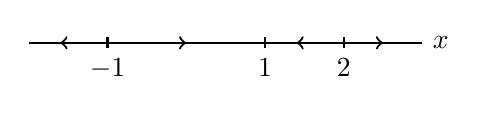
\begin{tikzpicture}[thick]
        % [scale=1.5]
        % \draw (-2, 0) -- (4, 0);
        %
        % \fill (-1, 0) circle (0.05);
        % \fill (1, 0) circle (0.05);
        % \fill (2, 0) circle (0.05);
        %
        % \node[label=below:{-1}] at (-1, 0) {};
        % \node[label=below:{1}] at (1, 0) {};
        % \node[label=below:{2}] at (2, 0) {};
        %
        % \draw [<-] (-1.5, 0) -- (-1.4, 0);
        % \draw [->] (-0.1, 0) -- (0, 0);
        % \draw [<-] (1.4, 0) -- (1.5, 0);
        % \draw [->] (2.4, 0) -- (2.5, 0);
        [scale=1.5]
        \DrawHorizontalPhaseLine[\(x\)]{-1, 1, 2}{0, 2.5}{-1.5, 1.5}
      \end{tikzpicture}
    \end{figure}

    This makes it clear that \(x = -1\) is a \textbf{source}, \(x = 1\) is a \textbf{sink}, and \(x = 2\) is a \textbf{source}.
  \end{solution}

  \pagebreak

  % Problem 1.5 #21
  \begin{problem}[Problem 1.5.21]
    A 600-liter tank initially contains 200 liters of water containing 10 kilograms of salt.
    Suppose that water containing 0.1 kilograms of salt flows into the top of the tank at a rate of 10 liters per minute.
    The water in the tank is kept well mixed, and 5 liters per minute are removed from the bottom of the tank.
    How much salt is in the tank when the tank is full?
  \end{problem}

  \begin{solution}
    Let \(x(t)\) be the amount of salt in the tank at time \(t\).
    Then the initial condition tells us that \(x(0) = 10\).
    We also let \(V(t)\) be the amount of water in the tank at time \(t\).
    Then \(V(t) = 200 + 5t\).

    Furthermore, we know the rate at which salt flows in and out of the tank.
    Then we have
    \begin{gather*}
      \frac{dx}{dt} = 10 (0.1) - \frac{5x}{V(t)} = 1 - \frac{x}{40 + t}.
    \end{gather*}
    Rearranging, we get the first order linear differential equation
    \begin{equation*}
      \frac{dx}{dt} + \frac{1}{40 + t} x = 1.
    \end{equation*}
    We solve for the integrating factor
    \begin{equation*}
      \mu(t) = \exp \left( \int \frac{1}{40 + t} dt \right) = 40 + t.
    \end{equation*}
    Multiplying both sides of the differential equation by the integrating factor yields
    \begin{equation*}
      (40 + t) \frac{dx}{dt} + x = 40 + t
    \end{equation*}
    or
    \begin{equation*}
      \frac{d}{dt}\left[ (40 + t) x \right] = 40 + t.
    \end{equation*}
    We can integrate both sides with respect to \(t\) to get
    \begin{equation*}
      (40 + t) x = 40t + \frac{t^{2}}{2} + C.
    \end{equation*}
    If we use our initial condition of \(x(0) = 10\), then we find \(C = 400\).
    Rearranging our above equation, we obtain a solution of
    \begin{equation*}
      x(t) = \frac{t^{2}  + 80t + 800}{2t + 80}.
    \end{equation*}
    Since the maximum capacity of the tank is 600 liters, the tank is full at time \(t = 80\).
    Finally, we find that \(x(80) = \frac{170}{3} \approx 56.667\).
    That is, the tank contains about 56.667 kilograms of salt when it is full.
  \end{solution}
\end{document}
